\section{Rule Language Specification}\label{sec:rule-language-specification}

The following code snipped \addref shows all upper level fields in the rule object.

\lstinputlisting[
language=json,
style=json,
caption={Rule root}
label={lst:rule-root}
]{code/rules/rule-root.json}

\section{Information Scope}\label{sec:information-scope}
Part of this work was
to identify billing-relevant information sources through expert interviews and research in the billing catalogs \addcite.
From a higher level perspective, all found information sources are part of the following domains:
\begin{itemize}
    \item The treatment documentation that contains all medical information of the treatment
    \item Treatment-independent patient information
    \item Treatment-independent practitioner information
    \item Patient history containing all previous billing positions
\end{itemize}




\subsection{Quantity Functions}\label{subsec:quantity-functions}

In the previous chapter we introduced the concept of a billing rule.

Not only which codes are part of the billing but also their quantity is highly important information.
In the previous section, we explained how the billing framework derives a set of applicable billing codes.
The result data type was essentially a set of billing codes.
In this section, we generalize the framework in such a way that it returns each code in combination with its quantity.

We extend the general rule structure by introducing the concept of quantity functions.
Similarly to rule conditions, quantity functions are evaluatable subcomponents of a rule.
The framework evaluates quantity functions of rules for a\code{RuleEvaluationInput}.
The result is an integer that indicates how often it should be billed in the billing.

\begin{equation}
    \label{eq:quantity-function-natural}
    f_{quantity}: \code{RuleEvaluationInput} \longrightarrow \mathbb{N}
\end{equation}

Billing code quantities typically rely on two types of billing information.
Subsection\ref{subsubsec:quantity-derivation-from-procedure-information} and\ref{subsec:quantity-derivation-from-durations} explain these sources.

\subsubsection{Quantity Derivation From Procedure Information}\label{subsubsec:quantity-derivation-from-procedure-information}

I derived the requirement for quantity functions from \goa{255: Injection, intra-articular or perineural}.
It is an example of a code, that is likely to appear in a billing with a quantity larger than one.

The so-called Spine Infiltration is a procedure, that includes injections into spine nerves.
Billing experts use \goa{255} for this medical service.
Procedure block \code{SpineInfiltrationMsg} represents this procedure.
However, \goa{255} typically applies once for each spine injection the practitioner actually provided.
Therefore, a spine infiltration can include multiple injections at different localizations.
The system should not only be able to derive \goa{255} for a provided spine infiltration, but should also be able to derive the correct quantity of \goa{255} codes.

To illustrate this example, it is worth mentioning that the human spine consists of three primary regions \cite{BOGDUK2016675}:
\begin{itemize}
    \item The cervical spine, the thoracic spine, and the lumbar spine.
    The cervical spine comprises the uppermost part of the spine, which is the neck and head.
    \item The thoracic spine, located in the middle, has twelve vertebrae attached to the rib cage, providing stability and structure to the upper body.
    \item Lastly, the lumbar spine at the lower back is made up of five larger vertebrae, designed to bear the body's weight and provide flexibility and movement.
\end{itemize}
Each region has well-defined localizations that can be targets for injections.
The \AVS stores the data of a spine infiltration in a \code{SpineInfiltrationMsg}procedure block.

The following code snipped displays a simplified version of it.
\lstinputlisting[
    language=protobuf3,
    style=protobuf,
    caption={Relevant localizations in a spine infiltration}
    label={lst:spineInfiltration},
]{code/proto/spineInfiltration.proto}


\code{SpineInfiltrationMsg} has a nested message\code{NerveRootBlockMsg}.
\code{NerveRootBlockMsg} contains the messages,\code{CervicalSpineMsg}\code{ThoracicSpineMsg} and\code{LumbarSpineMsg}.
These messages represent the before-mentioned sections of the human spine.
Each variable in these nested messages is of type \code{Laterality}and represents injections at the respective localization alongside the spine.
The laterality of an injection refers to the specific side or sides where the injection is administered in the spine localization.
This can be either on the left side, the right side, or on both sides.

To get the total number of injections, the system would need to peek into the nested messages \code{CervicalSpineMsg}, \code{ThoracicSpineMsg} and\ code{LumbarSpineMsg} and compute the total number of injections from the laterality values.
Additionally, the framework needs to be able to understand that \code{LATERALITY\_NONE} refers to zero and \code{LATERALITY\_LEFT} as well as\code{LATERALITY\_RIGHT} refer to one injection.
\code{LATERALITY\_BOTH} refers to two injections.
It is important to assign quantities to enum values.


\subsubsection{Quantity Derivation From Durations}\label{subsec:quantity-derivation-from-durations}

Many GOÄ codes specify not only a service content but also a time range.
If provided services exceed that time range the respective code can be billed more than once.

\goa{21: Incoming human genetic counseling, per commenced half-hour and session} is an example for such a code.
If the counseling takes one hour and 10 minutes, \goa{21} can be billed 3 times.
Similar codes are \goa{61: Assistance in the medical service of another doctor (Assistance), per commenced half-hour}
and \goa{85: Written expert opinion involving an effort exceeding the usual extent – possibly with scientific justification –, per commenced hour of work}
Codes that with that characteristic often end with \("\)per commenced hour\("\) or \("\)per commenced half-hour\("\) to indicate the time range.
Those are comparably simple cases.

\mete{Section D: Anesthesia Services} contains a specific class of edge case that use time ranges.

\goa{462: Combined anesthesia with endotracheal intubation, up to one hour} and \goa{463: Combined anesthesia with endotracheal intubation, each additional commenced half-hour}
both denote the same procedure provided, but as their names suggest, they distinguish between different periods of service provision.
\goa{462} is applicable only once per procedure.
On the other hand, code \goa{463} covers each additional half-hour beyond the initial hour.
Its billing number is variable and depends on the total duration of the anesthesia.
\goa{463} excludes the first hour of service provision, already covered under code \goa{462}.

The GOÄ distinguishes between \goa{462} and \goa{463} because of the following reasons.
\goa{462} covers both the induction and the maintenance of anesthesia for the first hour.
This is the most critical phase involving continuous administration of medication to make sure the patient remains asleep.
The time after the first hour typically requires only maintenance of anesthesia and is therefore less critical.
\goa{463} applies to subsequent commenced half-hours after the first hour and is therefore lower priced than \goa{462}.


Anesthesia services frequently use this pattern of code groups referring to the same provided procedure but distinguishing between service periods.
Equivalent examples are \goa{460/461}, \goa{476/477} and \goa{478/479}.
\goa{473, 474 and 475} are a more special example.
They refer to an initiation and monitoring of a continuous subarachnoid spinal anesthesia, again distinguishing between durations.
\goa{473} applies to durations shorter than five hours, \goa{474} to the subsequent five hours and \goa{475} applies once for the second and every subsequent day.

These examples lead to concrete requirements for the billing framework and underline the importance of \"quantity functions\".
They must be expressive enough to represent and manage the nuances of these examples.
Section\ref{sec:quantity-function-specification} illustrates how users can express these cases using the rule language.

\subsection{Partial Billing Quantitys}\label{subsec:partial-billing-quantitys}
In very special cases billing codes apply with a reduced quantity of points.

%There are at least two cases:
%\goa{D} is a surcharge for services provided on saturday, sunday and on holidays.
%If service provision happens during an opening hour, \goa{D} only applies with half the fee, though.
%This is also the case for surcharges \goa{E}, \goa{F}, \goa{G} and \goa{H} if \goa{51} is part of the billing, as well.
%
%The framework must be able to express these edge cases but does not allow any point value manipulations of billing codes.
%It solves this issue using quantity functions.
%In those cases the quantity function must be able to evaluate to 0.5 which results in the same fee reduction as required by the GOÄ specification.
%
%This requirement changes the formal definition given in formula \ref{eq:quantity-function-natural} to:
%\begin{equation}
%    \label{eq:quantity-function-real}
%    f_{quantity}: \code{RuleEvaluationInput} \longrightarrow \mathbb{R}^{+} \\ \left{0\right}
%\end{equation}
%Quantity function now evaluate


\subsection{The Condition Predicate}\label{subsec:the-condition-predicate}

In the following sections, we formally define the semantics of \RL and introduce its language features.
The syntax is pure JSON.
Additionally, we back up each language feature with use cases that lead to their implementation.
These requirements are the result of either conducted expert interviews or research in medical billing documents and catalogs.

%The condition object implements a condition in the rule definition mentioned in section \ref{sec:aspects-of-rule-based-systems}.
%The billing framework can evaluate a condition object for a so-called \code{RuleEvaluationInput} instance.
%It is essentially a data class that contains all information required by any of the following conditions to be evaluated.

\subsection{The Condition Triplet pattern}\label{subsec:the-condition-triplet-pattern}
As mentioned in section \addref rule-based systems require regular maintenance and rule updates.

As denoted in \addref one of the requirements for a rule-based system is extendability. \addcite
This does not only refer to the rules in the rule-base but also to the framework itself.
During the design of the Billing Framework I put great emphasis on extendability
by making use of the pattern illustrated in figure \ref{fig:condition-triplet-pattern}.

\begin{figure}
    \centering
    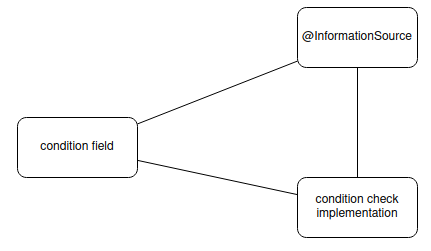
\includegraphics[width=0.75\linewidth]{./figures/condition-triplet-pattern}
    \caption{Generic illustration of the triplet pattern}
    \label{fig:condition-triplet-pattern}
\end{figure}

Adding a new condition type to the condition predicate of \RL requires the implementation of what I call the condition triplet pattern.

\paragraph{Condition Field}
Each condition type requires a meaningful keyword with a proper data type in the rule language schema.
Generally speaking, complicated condition features tremendously reduce user-friendliness.
Feedback from Dr. Bojko has shown that many simple condition fields are preferable to fewer, more complex ones, as the latter are more prone to errors.
A rule of thumb is to use flag-like boolean type fields whenever possible.

\paragraph{Information Source}
Each condition subscribes to one or more information sources.
An information source is a type of medical or administrative information that, as part of my research, I have identified as relevant for billing.
Billing-relevant information is information upon which the codes we want to derive depend.
Each Information source requires a fetch implementation, that fetches the data from other \AV services and makes sure the condition check implementation has access to it.

\paragraph{Condition Check Implementation}
Each condition field requires an actual condition implementation that expects a \code{RuleEvaluationInput} object as an input and returns the condition result.
\code{RuleEvaluationInput} objects are data classes that conveniently provide the data that represents fetched information sources required by the existing condition fields.
Section \addref describes them in more detail.

Figure \ref{fig:condition-triplet-pattern-instance-1} and \ref{fig:condition-triplet-pattern-instance-2} illustrate concrete implementations of the condition triplet pattern
for the condition fields \code{newBorn} and \code{minPatientAge}.
Both subscribe to the \code{@InformationSourcePatientAge} information source but have different condition check implementations.

\begin{figure}
    \centering
    \begin{subfigure}[b]{0.45\linewidth}
        \centering
        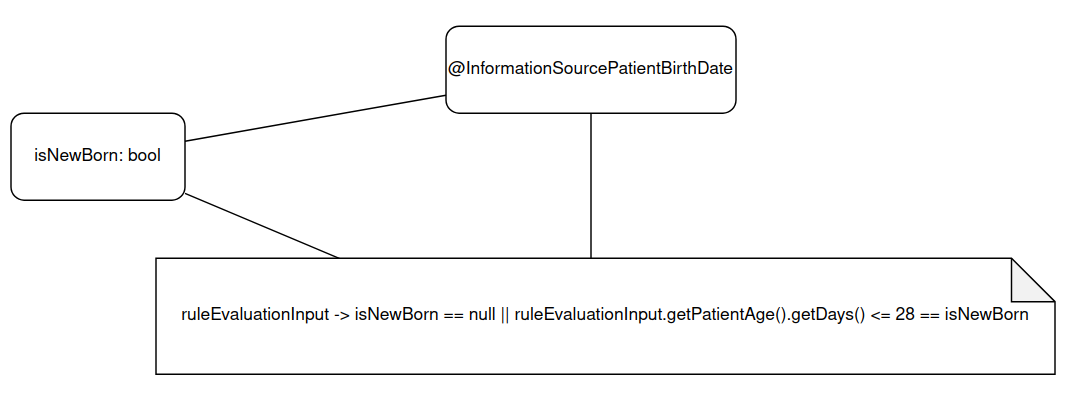
\includegraphics[width=\linewidth]{./figures/ctp-is-new-born}
        \caption{Condition Triplet pattern instance 1}
        \label{fig:condition-triplet-pattern-instance-1}
    \end{subfigure}
    % Adjust or remove the space between figures as needed
    \hspace{5mm} % This adds a bit of horizontal space between the figures
    \begin{subfigure}[b]{0.45\linewidth}
        \centering
        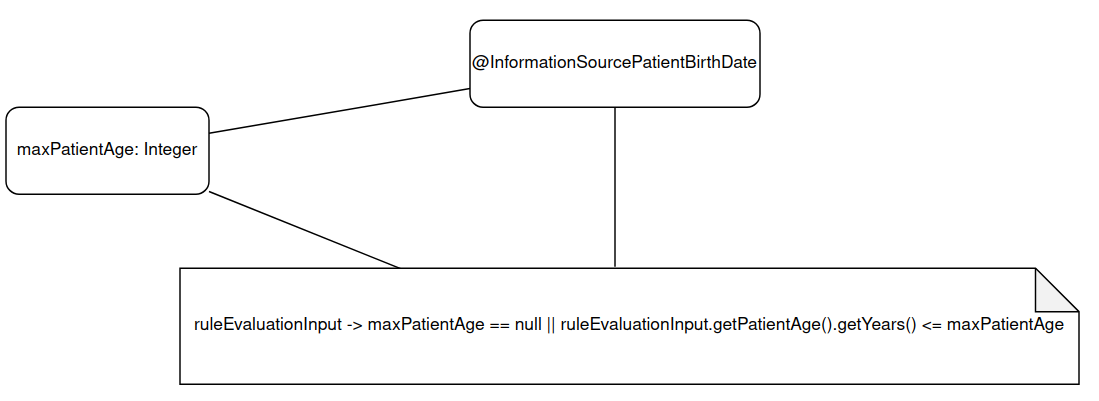
\includegraphics[width=\linewidth]{./figures/ctp-max-patient-age}
        \caption{Condition Triplet pattern instance 2}
        \label{fig:condition-triplet-pattern-instance-2}
    \end{subfigure}
    \label{fig:coffee}
\end{figure}
This section discusses the \code{condition} field of a rule.
Its value is a condition object with the following fields.

\subsection{Patient Related Conditions}\label{subsec:patient-related-conditions}

\paragraph{minPatientAge / maxPatientAge}
\code{minPatientAge} and \code{maxPatientAge} are integer fields that enable restrictions on the patient age.
Both fields store a number of years.
You can combine both to require the patient age to be within a certain age interval.

In medical practice, the age of a patient can significantly influence the complexity of a treatment.
In cases involving very young or very elderly patients, practitioners may encounter patient age specific challenges.
Due to these challenges, treatments may require more time, special care or other additional resources.
As a result, practitioners may apply billing multipliers to compensate for the additional effort.
This is why you can use the \code{minPatientAge} and \code{maxPatientAge} fields implement these types of multiplier justification rules.
There are also concrete GOÄ codes such as \goa{K1} and \goa{K2} that require the patient age.
The patient age is also highly relevant for various EBM codes, but already exists as structured conditions in the EBM catalog.
This is why using patient age conditions in EBM rules is redundant.
The information source for these two conditions is \code{@InformationSourcePatientAge}.

\paragraph{isNewBorn}
\code{isNewBorn} is syntactic sugar and a special case of the \code{maxPatientAge} condition.
It is a bool field that denotes whether a patient must be a newborn or not.
According to the GOÄ, babies that are at most 28 days old are newborns \cite{bruck1998kommentar}.
It is relevant for \goa{25: Initial newborn examination – if necessary including advice from the caregiver(s) –}, which is essentially a provision of a physical examination for newborns.
It can also be interesting for multiplier justifications.
The information source for these two conditions is \code{@InformationSourcePatientAge}.

\paragraph{patientSpeaksGerman/patientSpeaksEnglish}
\code{patientSpeaksGerman} and \code{patientSpeaksEnglish} are both boolean fields that denote whether the patients are able to communicate in the respective language.
Communication problems can increase the effort and time a treatment may require and are often used as justifications for multipliers which compensate for that.
\goa{4: taking a third-party medical history} covers an anemnesis that \todo{finish}
\code{patientSpeaksGerman} and \code{patientSpeaksEnglish} subscribe to the information source \code{@InformationSourcePatientLanguages}.

\paragraph{gender}
The \code{gender} condition is one of the most important condition types.
It is relevant for various EBM and GOÄ codes.
Similarly to patient age, gender conditions are already a structured part of the EBM catalog and do not need to be used in EBM rules.
\goa{27}, \goa{28},  GOÄ codes in section \mete{H}, Obstetrics and Gynecology, and GOÄ codes in \mete{Urology} are gender-specific.
Rules implementing these codes can use the \code{gender} condition.
It supports the string values \code{\"female\"}, \code{\"male\"} and \code{\"diverse\"}.
\code{gender} subscribes to the information source \code{@InformationSourcePatientGender}.


\paragraph{isPregnant}
The \code{isPregnant} condition is syntactic sugar for a specific case of the \code{requiredAnamnesisBlocks}
The following rules are equivalent.

\lstinputlisting[
    language=json,
    style=json,
    caption={\code{isPregnant} rule},
    label={lst:is-pregnant}
]{code/rules/specification/isPregnant.json}

A pregnancy can be reason for additionally required care or services during a treatment that is not related to the patient's pregnancy.
This is why it can be useful in multiplier justification rules.
It is also useful for \goa{23} which is applicable for an initial pregnancy-related examination.
\code{isPregnant} subscribes to the information source \code{@InformationSourceAnamnesisBlocks}.

\paragraph{isSober}
The \code{isSober} boolean condition describes the current state of the patient during the treatment.
A patient is considered non-sober when under the influence of alcohol or addictive substances.
\code{isSober} is effectively syntactic sugar for a specific use case of the \code{requiredAnamnesisBlocks} condition.
The following rules are equivalent
\lstinputlisting[
    language=json,
    style=json,
    caption={\code{is sober} rule},
    label={lst:is-sober}
]{code/rules/specification/isSober.json}


\paragraph{minNumberOfAllergies}
\code{minNumberOfAllergies} is a field that specifies the minimal number of allergies a patient requires.
From medical experts at \AV I have learned that a high number of allergies can make treatments more challenging for several reasons:
\begin{itemize}
    \item It may reduce the number of medical options as medications contain allergens or can produce them in specific environments.
    \item It can increase the complexity of the diagnostic process, as allergy reactions can mimic symptoms of other diagnoses.
    \item Patients with a high number of allergies require increased caution and care.
    Practitioners need to spend more time for history review and patient monitoring.
\end{itemize}
This makes \code{minNumberOfAllergies} a useful condition for multiplier justifications.
It subscribes to the information source \code{@InformationSourcePatientAllergies}

\subsubsection{Block Content Related Sub-rules}

A medical treatment consists of multiple stages of patient care.
Each stage has its specific aims and tools.
Anamnesis,
physical examination and procedures represent different stages of patient care and are highly relevant for billing.

\paragraph{Anamnesis}
Anamnesis is the first stage of a treatment.
Its purpose is to collect a detailed medical history from the patient\cite{lino2021medical}.
More specifically, it is about understanding the patient's general health conditions,
their lifestyle and previous patients' diagnoses.
If possible, the practitioner reviews available medical records,
interviews the patient directly or using a questionnaire\cite{zhang2011anamnevis}.

\paragraph{Physical Examination}
Anamnesis is followed by the Physical Examination.
In this practical stage, the practitioner assesses the current patient's conditions,
looking for further information about the patient's issues\cite{seidel2010mosby}.
The practitioner decides based on patient's symptoms which exact examinations are conducted.
Common examinations are checking of vital sings like blood pressure, pulse and temperature.

\paragraph{Procedures}
The procedure stage contains the actual patient-specific interventions that \todo

\paragraph{Block Contents}
As part of the Anamnesis, Physical Examination and Procedures stage,
the practitioner enters medical treatment specific information into the \AVS.
All three stages have separate documentation with a tree-like structure consisting of sections, cards and blocks.
Blocks are topic-related medical questionnaires that, depending on the patient's condition, the practitioner selects and fills out.
For example, the physical examination contains the section \mete{abdomen} that contains the \mete{liver} card.
The \mete{liver} card contains the blocks \mete{liverPalpation} and \mete{liverSize}.
Blocks are essentially small questionnaires for the practitioner with input fields to be filled out by the practitioner.
They play a huge role in treatment documentation and contain relevant medical information specific to this provided examination, procedure or anamnesis.
\code{LiverPalpation} is an example for an example for a physical block in the \code{liver} section.
A classic liver palpation examination involves answering the following questions \cite{wolf1990evaluation}:
\begin{itemize}
    \item Is the liver palpable?
    \item Is the liver texture soft or tender?
    \item Is the liver surface smooth or knotty?
    \item Is tenderness present?
    \item Are pulsations present?
    \item Is a hepato jugular reflux present?
\end{itemize}
Within the \AVS each block consists of meta-data such as timestamps, ids as well as a block content sub-object.
The \AVS defines several hundreds block contents for physical examination, anamnesis and procedures blocks.
It uses the object-relationship-mapping Hibernate to map all block content class definitions to database tables.
Each attribute of that class stores a questionnaire input entered by the practitioner.
Additionally, for each entity, there is a protobuf message definition enabling transmission of block content data from one service
to another one.
The protobuf messages of the block contents are the most important part of the structured data provided by \AV which the billing framework heavily relies on.
The protobuf message of \code{LiverPalpationMsg} looks like this:
\lstinputlisting[
    language=protobuf2,
    style=protobuf,
    caption={LiverPalpation protobuf messages}
]{code/proto/liverPalpation.proto}


The exact principle applies throughout the procedure and anamnesis stage as well.
A crucial part of the rule language is not only to check for present blocks in the treatment
but also to look inside the blocks and check for field values.
A GOÄ code might have as a condition that a liver palpation examination is part of the treatment and
the liver turned out to be palpable.
Or an OPS code should only be derived if a \code{ECG} procedure was provided and the
input field \code{telemetricExamination} inside its block has the value\true.
Logical combinations of such single field conditions may also occur.
Expressing such conditions in a well-defined and user-friendly way is an important requirement for the rule language.

\paragraph{Block Content Field Types}
A block content can contain information of different input types.
The billing framework must handle and validate each input type differently.
The most basic field types are boolean flags and numeric inputs.
The \AVS uses the following scalar wrapper protobuf messages for them:

\lstinputlisting[
    language=protobuf2,
    style=protobuf,
    caption={Scalar wrapper types}
]{code/proto/scalarWrapper.proto}

The purpose of wrapping scalars in custom protobuf messages is to make scalar default values distinguishable from missing data.
Initializing a protobuf message without explicitly setting the value of field has the consequence that the field gets initialized with its default value.
The default value for \code{int32} is 0.
If a gRPC server receives a protobuf message with an \code{int32} field set to 0, it does not know if the field was purposely initialized with 0 or not set at all.
Wrapping integers in \code{Int32W} messages makes this distinguishable.

Liver tenderness can either be present or not, which makes it a \code{BoolW} field.
The \AVS uses enumeration fields for inputs that have a limited number of predefined values
For example, the most frequently used enum type is \code{AbnormalitiesExaminationResult}.
It denotes the result of a specific examination, which can be either conspicuous or inconspicuous.

\lstinputlisting[
    language=protobuf2,
    style=protobuf,
    caption={\code{AbnormalitiesExaminationResult}}
]{code/proto/enum.proto}

Knowledge inputs are another important input type.
They serve similar purposes as enum types but are not hard-coded into the code base.
The system fetches them from a dedicated microservice that stores them in a MeiliSearch database.
Block content conditions are a powerful tool to make codes dependent on concrete medical information from anamnesis,
physical examination and procedures.

\todo{introduce nested objects, list objects}

\subsubsection{Time Related conditions}

\paragraph{procedureDurations}
Procedure durations are a crucial information source on which GOÄ codes as well as multiplier justifications rely on.
Anesthesia services such as \goa{460}, \goa{462}, \goa{473} and \goa{476} have a duration condition.
Procedures that took longer than expected are an important justification for billing multipliers.

\RL implements procedure duration conditions in a slightly different way compared to other condition fields.
Figure \ref{lst:min-max-duration} illustrates example usages of this feature.

\lstinputlisting[
    language=json,
    style=json,
    caption={\code{minDuration} and \code{maxDuration}},
    label={lst:min-max-duration}
]{code/rules/specification/minDuration.json}

Code \code{1} holds if the laryngoscopy takes at most 10 minutes.
Code \code{2} holds if the laryngoscopy takes between 10 and 20 minutes.
Code \code{3} holds if the laryngoscopy takes at least 20 minutes.

Both \code{\$minDuration} and \code{\$maxDuration} are fields that belong inside the procedure block object of the \code{requiredProcedureBlocks} field.
They start with a \"$\" sign character to mark them as special fields distinguishing them from ordinary procedure block content fields.
They are integer fields that denote a number of minutes.
A duration condition always refers to an existing procedure, which is why we write it directly into the respective procedure block condition.

\paragraph{isOutsideOfOfficeHours}
\code{isOutsideOfOfficeHours} is a boolean field that, if set to true, only evaluates to true if the treatment starts outside an official office hour.
Office hours are official time slots where practitioners provide medical services.
However, unanticipated urgencies and scheduling issues can be the reason for treatments provided outside of official office hours.
\goa{A}, \goa{B} and \goa{C} are a few examples for surcharges that apply in those cases.
This condition subscribes to \code{@InformationSourceTreatmentDate} and \code{@InformationSourceOfficeHours}.

\paragraph{daysOfWeek}
\code{daysOfWeek} is a list type condition that allows to set conditions on the week day.
Possible values inside the list are \code{\"monday\"}, \code{\"tuesday\"}, \code{\"wednesday\"}, \code{\"thursday\"}, \code{\"friday\"}, \code{\"saturday\"} and \code{\"sunday\"}.
Using any value outside of the weekdays leads to an error.
This condition is relevant for multiple GOÄ surcharges.
\lstinputlisting[
    language=json,
    style=json,
    caption={\code{minDuration} and \code{maxDuration}},
    label={lst:days-of-week}
]{code/rules/specification/daysOfWeek.json}
Code \code{1} holds if the treatment takes place on Sunday or Saturday.
The \code{daysOfWeek} condition subscribes to \code{@InformationSourceTreatmentDate}
This condition subscribes to \code{@InformationSourceTreatmentDate}.

\paragraph{timeOfDayRestrictions}
Using the \code{timeOfDayRestrictions} condition allows you to specify that the treatment should commence within any specified timeslot from a provided list of daily timeslots.
\lstinputlisting[
    language=json,
    style=json,
    caption={Code \code{1} holds if the treatment starts between 8 pm and 10 pm or between 6 am and 8 am},
    label={lst:time-of-day-restriction}
]{code/rules/specification/time-of-day-restrictions.json}
This condition subscribes to \code{@InformationSourceTreatmentDate}.

\subsection{Medical Coding Related Conditions}

\paragraph{minNumberOfDiagnosesInCurrentTreatment}
This field specifies the minimal number of diagnoses specified in this treatment.
One of the commonly used
In my research, I have learned that multimorbidity is a commonly used multiplier justification in the LMU dermatology.
Multimorbidity in medical terms defines the combination of two or more chronic medical conditions in an individual \cite{Reste2013The}.
These medical conditions may be can be a chronic disease, biopsychosocial factor or a somatic risk factor.
\code{minNumberOfDiagnosesInCurrentTreatment} is useful for implementing the multimorbidity multiplier justification rule.
The information source for this condition is \code{@InformationSourceTreatmentDiagnoses}.

\paragraph{requiredIcdCodes}

Icd codes are a highly important condition type.
They play an important role for flatrates, GOÄ codes and EBM codes.
To provide maximal flexibility, I implemented the concept of a logical code matching trees.

\lstinputlisting[
    language=json,
    style=json,
    caption={Logical Code matching tree rules},
    label={lst:logical-code-matching-tree}
]{code/rules/specification/codeMatchingTree.json}

Firstly, we define the term \"match\":
Let \( s_1 \) and \( s_2 \) be strings.
We say \( s_1 \) matches with \( s_2 \) if and only if \( s_2 \) is a prefix of \( s_1 \).
\begin{equation}\label{eq:matching}
    s_1 \text{ matches with } s_2 \iff \exists k \in \mathbb{N} \cup \{0\} : s_1 = s_2[0:k]
\end{equation}

Code \mete{1} holds if the current treatment has an ICD10 diagnose that matches with \mete{B20}.
Rule \mete{2} makes use of the logical \code{OR} operator and holds if the current treatment has a diagnose that matches with \mete{R07.0}, \mete{R07.1} or \mete{L}.

Note that \mete{L} is not a ICD code but chapter within the ICD catalog.
According to the definition \ref{eq:matching}, \mete{L} matches with every single ICD10 code in the \mete{L} chapter as all of them have the prefix \"L\".
This makes it easy to specify a large group of ICD10 codes in a logical code matching tree.
The ICD10 catalog has a tree structure that maintains the invariant that each node is a prefix of its child nodes.
In other words, each node matches its parent node.
Nested nodes are chapters, sections and subsections.
Leaf nodes are actual ICD10 codes.

Note the code range \mete{R47..R49} used in rule \mete{3}.
This indicates a discrete interval of codes between \mete{R47} and \mete{R49}, including both borders.
\mete{R47..R49} includes all codes that match with \mete{R47}, \mete{R48} and \mete{R49}.

Just as \code{minNumberOfDiagnosesInCurrentTreatment} it subscribes to the information source \code{@InformationSourceTreatmentDiagnoses}.
The practitioner manually selects diagnoses for the treatment.
This is why diagnoses are part of the treatment object and are straight-forward to fetch.

\paragraph{requiredOpsCodes}

\code{requiredOpsCodes} is equivalent to \code{requiredIcdCodes}, but applies to OPS codes.

The major difference here is how the system fetches OPS codes for this treatment.
Unlike diagnoses, the practitioner does not manually select OPS codes for the conducted procedures.
The billing experts at \AV have therefore requested that the billing framework should automatically derive OPS codes for treatments.
I solved this by defining OPS rules as a new rule type.
Any rule componenent that needs to derive OPS rules makes use of another rule component, namely \code{OpsRuleComponent}.
It implements data fetching for \code{InformationSourceOpsCodes} by deriving OPS codes using OPS rules.
Just as any rule type, billing experts are responsible for writing OPS rules, as well.

\paragraph{requiredTargetCode}

\code{requiredTargetCode} is similar to \code{requiredOpsCodes} and \code{requiredIcdCodes}, but has a few differences.
Firstly, it refers to the result set of the derivation.
Using this condition, you can implement that a code can only be billed with another set of codes.
Billing experts need this feature to implement \goa{K1} and \goa{K2} as well as other surcharge codes in the GOÄ.
Secondly, it defines the term \"match\" as a direct string equality.
\begin{equation}\label{eq:matching-string-equals}
s_1 \text{ matches with } s_2 \iff s_1 = s_2
\end{equation}
GOÄ, EBM and other possible code systems do not offer a hierarchical prefix tree structure that would allow definition \ref{eq:matching}.
Instead, \code{requiredTargetCode} uses definition \ref{eq:matching}.
Section \addref offers a more detailed description of how the condition checking for \code{requiredTargetCode} actually works.

\subsection{Previous Occurrence related Conditions}\label{subsubsec:previous-occurrence-related}

The \AVS internally structures treatments as follows:
A patient multiple billing cases, each one representing a quarter of the year.
During a quarter, a patient may have multiple visits.
Each visit has a reference to the respective billing case.
During a visit, a patient can have one or more treatments.
For example, a patient can have an operation followed by a medical round.
A medical round is a part of hospital routine where healthcare professionals visit patients at their bedsides,
assess the patient's medical condition and evaluate the treatment process.
The \AVS considers the operation and the medical round both as treatments linked to the same visit.
The smallest units in the hierarchy are the billing positions that are attached to a treatment.

Another important context within the private billing is the so-called treatment case.
A treatment case refers to the month following an initial treatment for a new medical condition \cite{bruck1998kommentar}.
Treatment cases can run in parallel if a patient has two unrelated medical conditions.
For example, if a patient visits the doctor for a knee injury on the 4th of May, a new treatment case starts for this knee injury and lasts until the 5th of June.
Every treatment related to this knee injury between the 4th of May and the 5th of June belongs to this treatment case.
If the patient visits the same doctor for a viral infection on the 10th of May, a second treatment case begins, lasting until the 11th of June.
Two treatment cases run in parallel because both medical conditions, the knee injury and the viral infection, are independent.
A treatment case always spans one month.
This is why if the patient receives treatment related to the knee one month after the initial treatment, a separate treatment case starts, even though both treatments are related to the same diagnosis.

Occurrence related condition types do not subscribe to any information source.
They do not require information from an external service but rely on the billing history of the patient.
The billing service stores billing positions in the local database.
Evaluating each of the following conditions includes a query on the

\paragraph{maxAmountPerBillingCase / maxAmountPerTreatmentCase / maxAmountPerVisit / maxAmountPerTreatment}
These condition fields set a limit on the code occurrences in the respective context.
The code is always the conclusion of the rule the condition is part of.
\todo{add example}


\paragraph{maxAmountPerDay / maxAmountPerMonth / maxAmountPerYear}
Similarly to the previous condition fields, \RL also allows setting limits for code usages in specific time spans.
\todo{add example}


\paragraph{onlyOncePerGoaeTreatmentCaseInCombinationWithSpecialServices}
This boolean condition field handles a highly specific but important edge-case involving \goa{1} and \goa{5}.
From the \PVC seminar, I have learned that within the same treatment case, both codes can be billed in combination with a special GOä code at most once.
A special GOÄ code is a code whose numeric number is higher or equal to 200.
This means within the same treatment case \goa{1} can be billed as often as possible, but only once in combination with any code larger than 200.
The same holds for \goa{5}.

\subsection{Service Performer related Conditions}

\paragraph{performerIsDoctor}
The \code{performerIsDoctor} condition is a boolean condition field that allows to impose conditions on the practitioner type.
The current version of the \AVS supports the following practitioner types:

\lstinputlisting[
    language=protobuf2,
    style=protobuf,
    caption={\code{AbnormalitiesExaminationResult}},label={lst:AbnormalitiesExaminationResult}]{code/proto/roleTypes.proto}

Given the rules in code snippet \ref{lst:performerIsDoctor}, \code{code1} would hold if the practitioner had the role \code{ROLE\_TYPE\_DOCTOR}
or \code{ROLE\_TYPE\_HEAD\_DOCTOR}.
Otherwise, \code{code2} would hold.
This condition is relevant for \goa{1} and \goa{2}, which are only applicable by doctors.

\lstinputlisting[
    language=protobuf2,
    style=protobuf,
    caption={\code{AbnormalitiesExaminationResult}},
    label={lst:performerIsDoctor}
]{code/rules/specification/performerIsDoctor.json}

\subsection{Conflict Conditions}\label{subsec:conflict-conditions}
Conflict conditions are special fields that the framework cannot evaluate during the ordinary rule evaluation phase.
The reason for that is the these fields require the final rule evaluation set as an input, which is obviously not known during the rule evaluation phase.
The framework does not define a information source for this type of information.
Instead, these fields receive a special handling in a separate derivation stage described in section \addref.

\paragraph{singleBillingPosition}
\code{singleBillingPosition} is a special condition type that if set to \true only evaluates to \true if it is the only code in the derivation result.
It is relevant for \goa{3}.
This condition does not subscribe to any information sources.

\paragraph{singleBillingPositionIfPractitionerIsDoctor}
\code{singleBillingPositionIfPractitionerIsDoctor} is an extension of of \code{singleBillingPosition}
This admittedly highly specific boolean condition field behaves as follows:

\[
    \code{\{singleBillingPositionIfPractitionerIsDoctor : true\} = \true} \leftrightarrow \code{\{practitionerIsDoctor : true\} = \false} \land \code{\{singleBillingPosition : true\} = \true}
\]


This condition subscribes to \code{@InformationSourcePractitionerType}.


\todo{finish this}

Even though this condition  condition field is admittedly very specific

that if set to true only evaluates to \true if it is the code in the derivation result.
It evaluates to true if the practitioner is not a doctor or the conclusion code is the only code in the derivation result.
This condition field requires special handling but also subscribes to information source \code{@InformationSourcePractitionerType}.

\paragraph{excludedCodes}
This condition field expects a list of conclusions as a value.
A rule using the \code{excludedCodes} field evaluates to false if any code in the \code{excludedCodes} list is a derivation result.
This


\subsection{Miscellaneous Conditions}\label{subsec:miscellaneous-conditions}

\paragraph{isCareRound / isMedicalRound}
\code{isCareRound} and \code{isMedicalRound} are boolean conditions that enable you to check if the treatment is a care / medical rounds.
\goa{46}, \goa{48} and \goa{50} are a few examples for services that require that information.
Both fields subscribe to the information source \code{@InformationSourceTreatmentType}


\subsection{The Multiplier Function}\label{subsec:the-multiplier-function}
The multiplier justification rule type does not use the concept of a quantity.
They require \code{condition} blocks to make them derivable for certain conditions.
Additionally, we also want to compute suggested multiplier values dynamically from the environment.
This is why I introduced the \code{multiplier} field, which is very similar to the previously introduced \code{quantity} field.
Both make use of numeric function expressions that allow for dynamic computation from their environment.

In contrast to quantity functions, a multiplier expression returns a positive floating point number with two decimal places.

In this subsection, we illustrate this concept using the following example.
From Dr. Sahra Bojko I have learned that regular laryngoscopies should take at most 20 minutes.
We can apply a duration related multiplier for laryngoscopies that exceed this duration.
The longer the laryngoscopy takes, the greater should be the value of the multiplier for the provided service.
One way of implementing this is by declaring multiple multiplier justification rules applying to different time intervals.

\clearpage
\lstinputlisting[
    language=json,
    style=json,
    caption={Step multiplier function},
    label={lst:multiplier-justification-function-steps}
]{code/rules/specification/multiplier-expression-steps.json}

All three rules logically exclude themselves due to the duration intervals in their \code{laryngoscopy} block conditions.

This implements the following step function declared in equation \ref{eq:multilier-justification-step-function} and illustrated in figure \ref{plot:multiplier-justification-step-function}.

\begin{equation}\label{eq:multilier-justification-step-function}
    f(x) =
    \begin{cases}
        1.5 & \text{for } 20 \leq x < 30, \\
        2.5 & \text{for } 30 \leq x < 40, \\
        3.5 & \text{for } x \geq 40.
    \end{cases}
\end{equation}

\begin{center}
    \label{plot:multiplier-justification-step-function}
    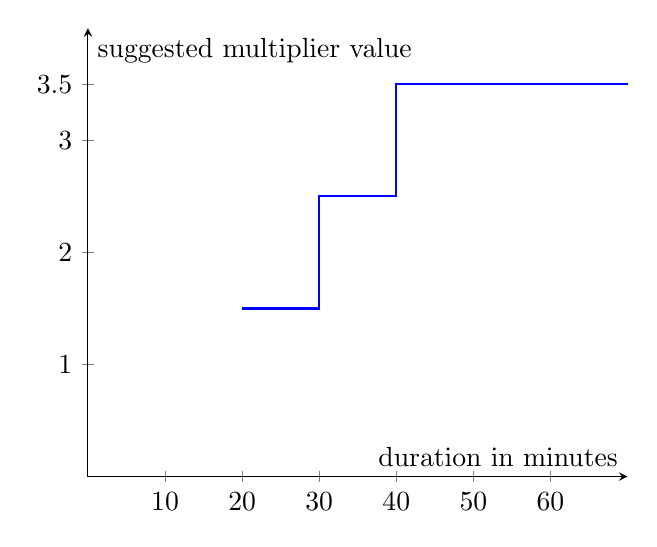
\begin{tikzpicture}
        \begin{axis}
        [
            axis lines=middle,
            xlabel={duration in minutes},
            ylabel={suggested multiplier value},
            xmin=0, xmax=70,
            ymin=0, ymax=4,
            xtick={10,20,30,40,50,60},
            ytick={0,1,2,3,3.5},
            clip=false,
            domain=20:75,
            samples=100,
        ]
            \addplot+[no marks, blue, thick, const plot] coordinates {(20,1.5) (30,2.5) (40,3.5) (70,3.5)};
        \end{axis}
    \end{tikzpicture}
\end{center}

Another more compact way to implement this is using a single rule with a more sophisticated multiplier expression.
Formula \ref{eq:bounded-linear-multiplier-function} is a valid choice for a multiplier function.

\begin{equation}
    \label{eq:bounded-linear-multiplier-function}
    f: \left[20, \infty\right) \rightarrow \left[ 1, \infty \right) : d \mapsto \min\left( 3.5, \frac{5}{40} d - \frac{3}{2} \right)
\end{equation}


Code snippet \ref{lst:multiplier-justification-function-linear} illustrates a rule that implements this multiplier function.
Note that the \code{condition} assures that the rule only applies to treatments with a provided laryngoscopy that took at least \code{20} minutes.
This sets the domain of the function to $\left[20, \infty\right)$.
This way inside, we can inside the \code{multiplier} block safely assume that the duration is greater or equal to 20.

\lstinputlisting[
    language=json,
    style=json,
    caption={Bounded linear multiplier function},
    label={lst:multiplier-justification-function-linear}
]{code/rules/specification/multiplier-expression-linear.json}


\begin{center}
    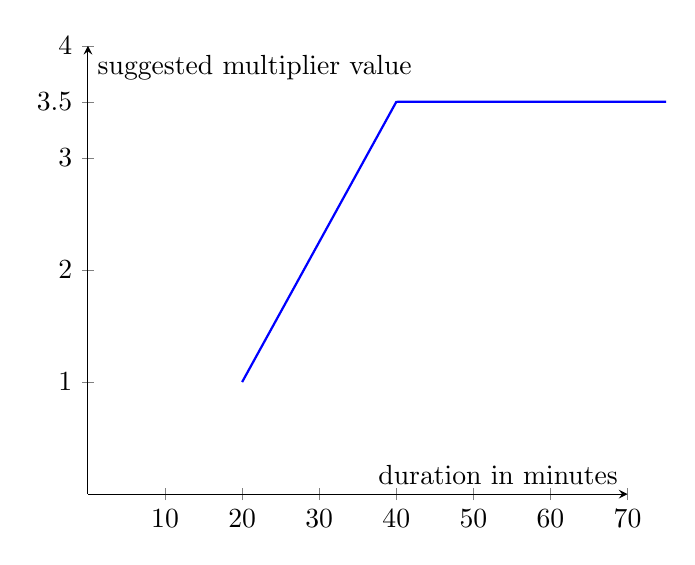
\begin{tikzpicture}
        \begin{axis}
        [
            axis lines=middle,
            xlabel={duration in minutes},
            ylabel={suggested multiplier value},
            xmin=0, xmax=70,
            ymin=0, ymax=4,
            xtick={0,10,20,30,40,50,60,70},
            ytick={0,1,2,3,3.5,4},
            clip=false,
            domain=20:75,
            samples=100,
        ]
            \addplot+[no marks, blue, thick] {min(5/40*x - 1.5, 3.5)};
        \end{axis}
        \label{plot:linear-mul-just}
    \end{tikzpicture}
\end{center}

Plot \ref{plot:linear-mul-just} illustrates the graph for the multiplier function.

For ordinary laryngoscopies that take less than 20 minutes, the multiplier justification rule does not match at all.
Note that with increasing laryngoscopy duration, the suggested multiplier linearly increases between 20 and 40 minutes.
For very unlikely cases where complications are so severe that the laryngoscopy takes more than 40 minutes, the rule suggests the maximum multiplier value of 3.5.


